% !TeX root = ../../thesis.tex
\chapter{Advanced model with kinetics}\label{ch:kinetics}


\begin{shaded}
This chapter is based on a manuscript prepared to be submitted:\\
M. Barzegari, C. Wang, S.V. Lamaka, G. Zavodszky, and L. Geris, ``Interface-coupled multiphysics computational modeling of local pH changes during the biodegradation of magnesium biomaterials.''
\end{shaded}

\section{Introduction}

Mg is the most studied biodegradable metal \cite{Liu2019,Zheng2014,Chen2014,Zhang2013}, on which many research groups have performed valuable biodegradation studies \cite{Esmaily2017,Li2016,Atrens2020,Kirkland2012}. The biodegradation behavior of Mg is investigated in \textit{in vitro} corrosion tests, in which the selection of the corrosive media plays an important role since it affects the underlying chemical reactions \cite{Mei2020}. By considering the main application of the biomaterial, which can be tissue engineering scaffolds, vascular stents, or orthopedic fixation implants, the corrosive media can be selected to be a representative of the service environment. The most basic form of the medium is a saline (NaCl) solution, in which the degradation rate is the highest possible \cite{Mei2020}. More complex solutions can be used to mimic the behavior of the body environment by taking into account additional body fluid components, the most popular of which are Ringer's solution, \gls{PBS} (phosphate buffered saline), \gls{SBF}s (simulated body fluids), \gls{HBSS} (Hank's balanced salt solution), and Earle's balanced salt solution (\gls{EBSS}) \cite{Mei2020}. Adding more organic components to the solution will make it ready to simulate cell culture conditions. The common media for this purpose are \gls{MEM} (Minimum Essential medium) and \gls{DMEM} (Dulbecco's modified Eagle's medium) \cite{Mei2020}.

Various studies have already investigated the effect of different components in the aforementioned corrosive media on the degradation behavior of Mg materials \cite{Mei2019,Zeng2014,Johnston2017, Lamaka2018,Mei2019a}. A typical composition of "simulated body fluid" solutions (such as \gls{SBF}, \gls{HBSS}, and \gls{EBSS}) is chloride, carbonate, phosphates, sulfate, and calcium. The individual effect of these components on the rate of degradation of Mg has been extensively studied, in which it has been observed that carbonate and phosphate slow down the rate while the effect of sulfate is negligible \cite{Johnston2017,Mei2019a}. The concentration of $\mathrm{HCO}_{3}^{-}$ affects the pH buffering capacity and the degradation rate of Mg simultaneously \cite{Xin2011}.

The effect of calcium ions is more complex because it has been found that $\mathrm{Ca}^{2+}$ doesn't contribute to the Mg corrosion directly \cite{Willumeit-Roemer2019}, but a mixed effect of $\mathrm{Ca}^{2+}$, $\mathrm{Mg}^{2+}$, $\mathrm{HCO}_{3}^{-}$, and $\mathrm{H}_{2} \mathrm{PO}_{4}^{-} / \mathrm{HPO}_{4}^{2-}$ forms a co-precipitation layer on the corroded surface of Mg, slowing down the corrosion rate of commercially pure Mg as well as of some Mg alloys \cite{Mei2019,Lamaka2018}. It has also been reported that although various Mg alloys show different intrinsic degradation behavior in NaCl solution, they possibly behave similarly in simulated body fluids \cite{Agha2016,Mei2019a}. Since the humoral regulations inside the human body control the changes in pH of body fluids, it is common to use pH buffers to mimic a similar condition, but it should be taken into account that buffering solutions may affect the degradation rate of Mg \cite{Cui2017,Kannan2017} and may also delay the formation of the precipitate layer \cite{Lamaka2018}. An alternative solution to address this issue is to use natural pH buffers such as $\mathrm{HCO}_{3}^{-}/\mathrm{CO}_{2}$, an option that is commonly used for immersion tests under cell culture conditions. In this situation, an equilibrium between $\mathrm{H}_{2} \mathrm{CO}_{3}\left(\mathrm{CO}_{2}\right)$, $\mathrm{HCO}_{3}{ }^{-}$, and $\mathrm{CO}_{3}{ }^{2-}$ keeps the pH constant. As a result, using simulated body fluids for corrosion tests without additional synthetic pH buffers is still acceptable \cite{Lamaka2018,Mei2019a}.

The major reactions occurring in simulated body fluids can be written as:
\begin{equation}
\mathrm{Mg}+2 \mathrm{H}_{2} \mathrm{O} \rightarrow \mathrm{Mg}(\mathrm{OH})_{2}+\mathrm{H}_{2}
\end{equation}
\begin{equation}
2 \mathrm{Mg}+2 \mathrm{H}_{2} \mathrm{O}+\mathrm{O}_{2} \rightarrow 2 \mathrm{Mg}(\mathrm{OH})_{2}
\end{equation}
\begin{equation}
5 \mathrm{Ca}^{2+}+3 \mathrm{PO}_{4}^{3-}+\mathrm{OH}^{-} \rightarrow \mathrm{Ca}_{5}\left(\mathrm{PO}_{4}\right)_{3} \mathrm{OH}
\end{equation}
\begin{equation}
\mathrm{Ca}^{2+}+2 \mathrm{OH}^{-} \rightarrow \mathrm{Ca}(\mathrm{OH})_{2}
\end{equation}
\begin{equation}
\mathrm{Mg}^{2+}+\mathrm{CO}_{3}^{2-} \rightarrow \mathrm{MgCO}_{3}
\end{equation}
\begin{equation}
\mathrm{Ca}^{2+}+\mathrm{CO}_{3}^{2-} \rightarrow \mathrm{CaCO}_{3}
\end{equation}
\begin{equation}
 3 \mathrm{Mg}^{2+}+2 \mathrm{PO}_{4}^{3-} \rightarrow \mathrm{Mg}_{3}\left(\mathrm{PO}_{4}\right)_{2}
\end{equation}
\begin{equation}
\mathrm{CO}_{3}^{2-}(a q)+H^{+}(a q) \rightarrow \mathrm{HCO}_{3}^{-}(a q)
\end{equation}
\begin{equation}
P O_{4}^{3-}(a q)+H^{+}(a q)\rightarrow \mathrm{HPO}_{4}^{2-}(a q)
\end{equation}

The protection layer is formed on the corroded surface as a hydroxyapatite-like precipitation according to the following reaction \cite{Atrens2015,Song2009,Silva2018,Jiang2019}:
\begin{equation} \label{eq:kinetics_hydrox_react}
\begin{aligned}
m \mathrm{Mg}^{2+}+n \mathrm{Ca}^{2+}&+x \mathrm{H}_{2} \mathrm{PO}_{4}^{-} / \mathrm{HPO}_{4}^{2-}+y \mathrm{HCO}_{3}^{-}+z \mathrm{OH}^{-}\\
& \rightarrow \mathrm{Mg}_{m} \mathrm{Ca}_{n}\left(\mathrm{PO}_{4}\right)_{x}\left(\mathrm{CO}_{3}\right)_{y}\left(\mathrm{OH}^{-}\right)_{z}
\end{aligned}
\end{equation}

In fact, the similarity in corrosion behavior of various Mg alloys in \gls{SBF} solutions is due to the similar composition of this quasi-protective layer, a mechanism that doesn't occur in NaCl solution, leading to a more apparent difference in degradation rate between Mg alloys. The composition of the formed hydroxyapatite-like precipitation layer is close to the ones found \textit{in vivo} \cite{Mei2020}. Additionally, local pH measurements in \gls{HBSS} and \gls{SBF} show that, in contrast to saline solutions, the local pH value is not alkaline \cite{Lamaka2018,Mei2021}. This has been reported for hydrodynamics situations, under which the medium composition is kept constant by replacing the consumed ions by means of fluid flow.

Building mathematical and computational models of the biodegradation process in complex buffered solutions can help save the resources required to perform \textit{in vitro} tests, but the details of the aforementioned chemistry are challenging to capture in a mechanistic model. Few attempts have been made to model the underlying chemical reactions in \gls{SBF} solutions \cite{Hoche2014,Dolgikh2019,Zeller-Plumhoff2022}, but due to the complexity of the resulting mathematical models, it is not feasible to extend them to 3D and real-world cases, like for simulation of the degradation of biomedical implants. In the case of data-driven approaches \cite{Zeller-Plumhoff2021}, the applicability is limited to the studied conditions, making it difficult for developed models to achieve high extensibility and generalizability. 

In this chapter, a detailed mathematical model is presented to extend the work discussed in previous chapters \cite{Barzegari2021}, in which a mechanistic model of the biodegradation process is coupled with a thermodynamics-based code to predict local interfacial biodegradation of Mg in \gls{HBSS} solutions. The local pH changes are the validation criterion to compare the simulation results with experimental ones. Besides other parameters affecting the Mg biodegradation mechanism, monitoring the pH changes at the degradation interface has proved to be significant due to its direct effect on the formation and stability of the degradation products layer \cite{Gonzalez2021}.


\section{Methods}

\subsection{Experimental setup}

\newglossaryentry{UHP}{name={UHP},description={ultra-high pure}}

In this study, the corrosion tests were performed on ultra-high pure (\gls{UHP}) and commercially pure (\gls{CP}) Mg in hydrodynamics conditions. The elemental composition of the used materials is shown in Table \ref{tab:kinetics_alloys_composition}, measured by Atomic Absorption Spectrometer (AAS). The samples were prepared as rod shapes with a diameter of $2\text{mm}$ mounted in epoxy resin with a disc shape. The electrolyte used for corrosion tests was commercial \gls{HBSS} (ThermoFisher Scientific, no. 14025100), the composition of which is presented in Table \ref{tab:kinetics_electrolyte_composition}.


\begin{table}[t]
\caption[The elemental composition of highly-pure and commercial-pure Mg]{The elemental composition of ultra-high pure and commercial pure Mg used for performing corrosion experiments (percentages)}
\medskip
\centering
\begin{tabular}{lcccccc}
\hline & {Fe} & {Si} & {Mn} & {Al} & {Cu} & {Ni} \\
\hline { \gls{CP}-Mg } & 0.03420 & 0.0001 & 0.00237 & 0.00402 & 0.00037 & <0.0002  \\
{ \gls{UHP}-Mg } & 0.0012 & <0.0001 & 0.00037 & 0.00291 & <0.0001 & <0.0002
\end{tabular}
\label{tab:kinetics_alloys_composition}
\end{table}

\begin{table}[h]
\caption[Chemical composition of the HBSS electrolyte]{Chemical composition of the \gls{HBSS} electrolytes used to perform corrosion tests for local pH measurements.}
\medskip
\centering
\begin{tabular}{cc}
\hline
{Components} & {mM} \\
\hline
$\mathrm{KCl}$ & 5.33 \\
$\mathrm{KH}_{2} \mathrm{PO}_{4}$ & 0.44 \\
$\mathrm{NaHCO}_{3}$ & 4.17 \\
$\mathrm{NaCl}$ & 137.9 \\
$\mathrm{Na}_{2} \mathrm{HPO}_{4}$ & 0.34 \\
$\mathrm{CaCl}_{2}$ & 1.26 \\
$\mathrm{MgCl}_{2} \cdot 6 \mathrm{H}_{2} \mathrm{O}$ & 0.49 \\
$\mathrm{MgSO}_{4} \cdot 7 \mathrm{H}_{2} \mathrm{O}$ & 0.41 \\
$\mathrm{D}-\mathrm{Glucose}$ & 5.56 \\
\hline

\end{tabular}
\label{tab:kinetics_electrolyte_composition}
\end{table}

\newglossaryentry{RT}{name={RT},description={room temperature}}

Local pH measurements were performed using a glass-type pH microelectrode with a tip diameter of $10\mu\text{m}$ (Unisense, pH-10). The electrode was positioned above the sample at a distance of $50\pm3\mu\text{m}$. At this distance, a line scan mapping routine was performed to obtain the horizontal pH profiles, in which a specimen-centered area ($3000 \times 3000 \mu\text{m}$, which was used as the simulation domain as well) was mapped with the step length of $100\mu\text{m}$. The sampling interval was 3 s, the result of which was a total duration of approximately 1 hour to scan the area. Similarly, the vertical pH profiles were scanned starting at the height of $50\mu\text{m}$ above the midpoint of the specimen up to $500\mu\text{m}$ in the bulk medium. Fig. \ref{fig:kinetics_setup} demonstrates the setup of the experiment schematically, in which the flow enters the chamber from the left with a rate of $1.0\text{mL.min}^{-1}$ (Medorex TL15E peristaltic pump) and leaves it to the right. The tests were performed independently at room temperature (\gls{RT}, $22 \pm 2$ in an air-conditioned lab) and $37^{\circ}\text{C}$ (Thermo Scientific SAHARA S13).


\begin{figure}[h]
\centering
\medskip
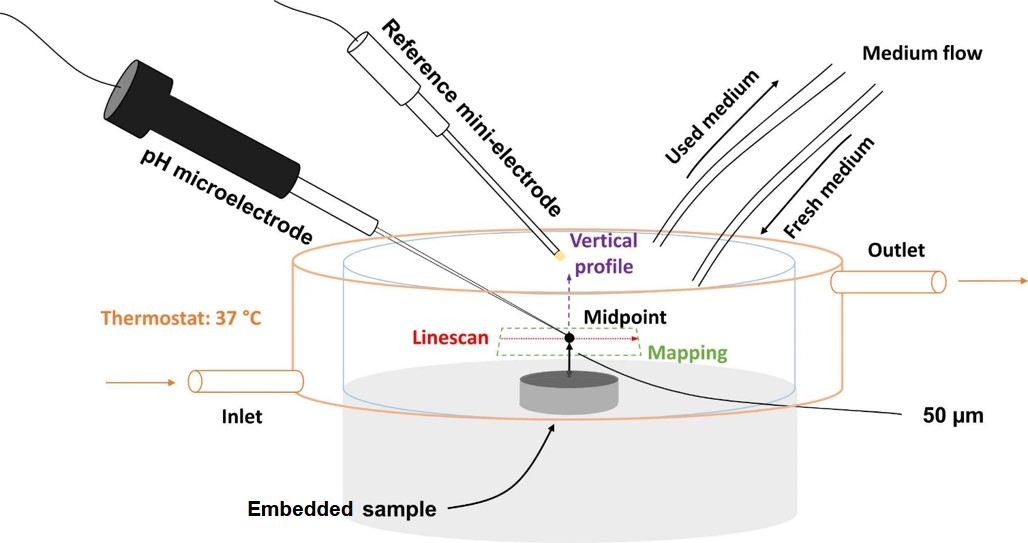
\includegraphics[width=0.9\textwidth]{setup.jpg}
\caption[Experimental setup for validating the coupled biodegradation model]{Experimental setup for validating the coupled biodegradation model} \label{fig:kinetics_setup}
\end{figure}

\newglossaryentry{FIB}{name={FIB},description={focused ion beam}}
\newglossaryentry{SEM}{name={SEM},description={scanning electron microscope}}
\newglossaryentry{EDX}{name={EDX},description={energy-dispersive X-ray}}

The \textit{in vitro} cross-section morphology of the specimens was characterized using a dual beam \gls{FIB}/\gls{SEM} platform (LYRA3 TESCAN) equipped with an \gls{EDX} system (Oxford Inca with a silicon drift detector), the result of which was used to compare qualitatively with the simulation predictions.

\subsection{Computational model construction}

The computational model in the current study comprises three coupled modules:
\begin{enumerate}
\item
An extended version of the mechanistic biodegradation model based on our previous work \cite{Barzegari2021} to obtain Mg and hydroxide ions distributions and the initial formation of the protective layer based on the modeling hypotheses.
\item
A thermodynamics-based simulation to estimate the concentration of various components of the electrolyte in regions close to the surface of the sample based on the calculated pH of module 1.
\item
A module to link the former two, calculating the hydroxyapatite-like precipitation concentration, in which calculated pH values were transferred from module 1 to module 2 for each node of the computational mesh to calculate the concentration of ions depending on the computed local pH and transfer back the calculated precipitation concentration to module 1.
\end{enumerate}

Fig. \ref{fig:kinetics_modules} shows a schematic representation of the coupled modules and the way that simulation data are being transferred between them.

\begin{figure}[h]
\centering
\medskip
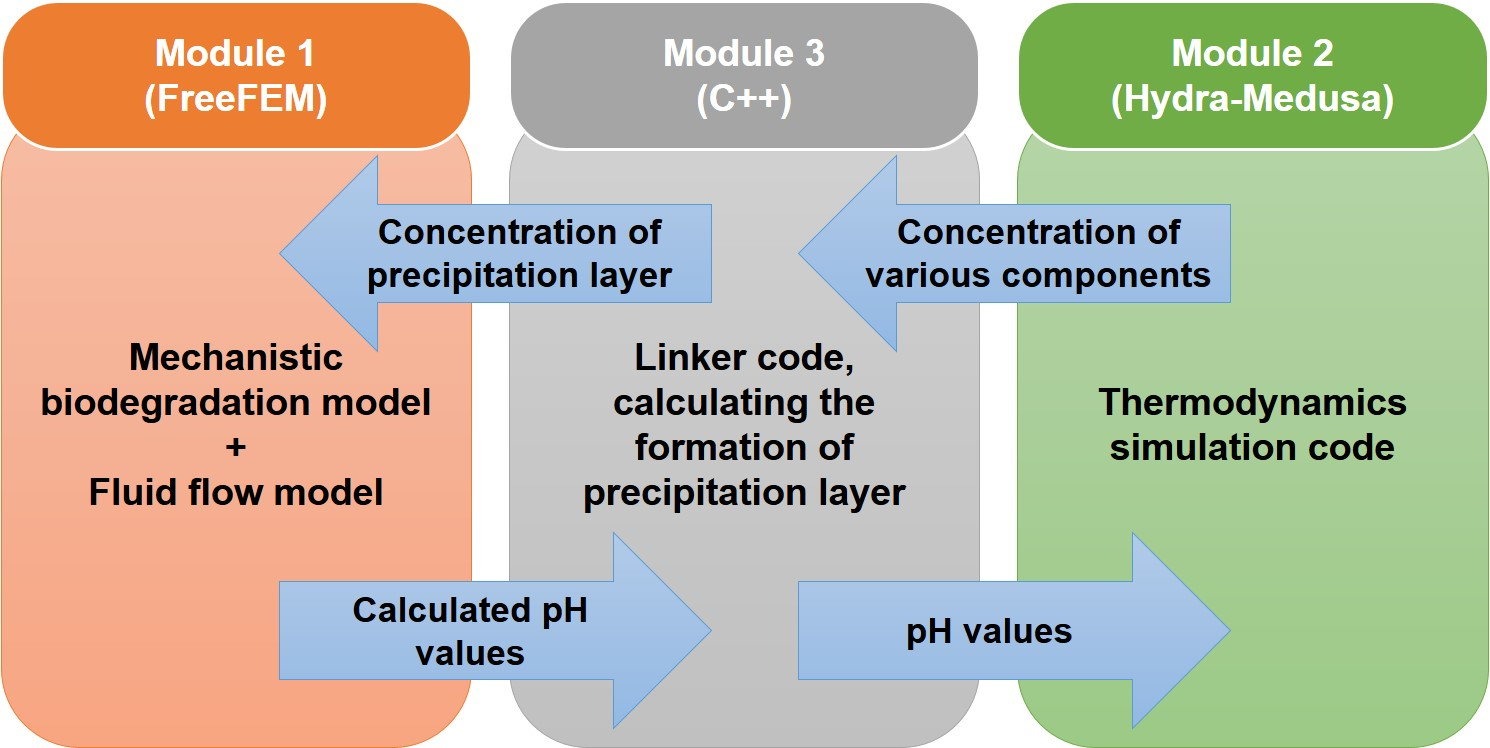
\includegraphics[width=\textwidth]{modules.jpg}
\caption[Schematic representation of the coupled modules for modeling of local pH changes]{Schematic representation of the coupled modules for modeling of local pH changes, showing how they are connected as well as the programming languages and tools used for the implementation.} \label{fig:kinetics_modules}
\end{figure}

The computational biodegradation model (module 1) was developed by deriving a set of reaction-diffusion-advection equations from the chemistry of the corrosion of Mg in hydrodynamics conditions. The following basic reactions are captured by this model, which is an extension of our previous contribution \cite{Barzegari2021} as the overall process is described in more detailed equations:
\begin{equation} \label{eq:kinetics_oxidation_react1}
\mathrm{Mg}+2 \mathrm{H}_{2} \mathrm{O} \stackrel{k_{0}}{\rightarrow} \mathrm{Mg}^{2+}+\mathrm{H}_{2}+2 \mathrm{OH}^{-}
\end{equation}
\begin{equation} \label{eq:kinetics_oxidation_react2}
\mathrm{Mg}^{2+}+2 \mathrm{OH}^{-} \stackrel{k_{1}}{\rightarrow} \mathrm{Mg}(\mathrm{OH})_{2}+\mathrm{H}_{2}
\end{equation}
\begin{equation} \label{eq:kinetics_break_react}
\mathrm{Mg}(\mathrm{OH})_{2}+2 \mathrm{Cl}^{-} \stackrel{k_{2}}{\rightarrow} \mathrm{Mg}^{2+}+2 \mathrm{Cl}^{-}+2 \mathrm{OH}^{-}
\end{equation}
\begin{equation} \label{eq:kinetics_break_react_mgo}
\mathrm{MgO}+ \mathrm{Cl}^{-} + \mathrm{H}_{2} \mathrm{O} \stackrel{k_{2}}{\rightarrow} \mathrm{Mg}^{2+}+ \mathrm{Cl}^{-}+ 2\mathrm{OH}^{-}
\end{equation}

The following state variables hold the concentration of various basic ions involved in reactions described by Eqs. \ref{eq:kinetics_oxidation_react1}, \ref{eq:kinetics_oxidation_react2}, \ref{eq:kinetics_break_react}, and \ref{eq:kinetics_break_react_mgo}:
\begin{equation} \label{eq:kinetics_state_vars_film}
\begin{aligned}
&C_{\mathrm{Mg}} = C_{\mathrm{Mg}}(\mathbf{x},t), \quad C_{\mathrm{Mg}_\mathrm{[s]}} = C_{\mathrm{Mg}_\mathrm{[s]}}(\mathbf{x},t), \quad C_{\mathrm{Mg}(\mathrm{OH})_{2}} = C_{\mathrm{Mg}(\mathrm{OH})_{2}}(\mathbf{x},t)  \\
&C_{\mathrm{Cl}} = C_{\mathrm{Cl}}(\mathbf{x},t), \quad C_{\mathrm{OH}} = C_{\mathrm{OH}}(\mathbf{x},t) \quad \mathbf{x} \in \Omega \subset \mathbb{R}^{3}
\end{aligned},
\end{equation}

Additionally, two more state variables are needed to couple the models, representing the calculated concentration of the hydroxyapatite-like precipitation as well as the cumulative layer concentration:
\begin{equation} \label{eq:kinetics_state_vars}
C_{\mathrm{Hydrox}} = C_{\mathrm{Hydrox}}(\mathbf{x},t), \quad C_{\mathrm{Film}} = C_{\mathrm{Film}}(\mathbf{x},t) \quad \mathbf{x} \in \Omega \subset \mathbb{R}^{3},
\end{equation}
where the total film concentration can be calculated as:
\begin{equation} \label{eq:kinetics_film_cumulative}
C_{\mathrm{Film}} = C_{\mathrm{Hydrox}} + C_{\mathrm{\mathrm{Mg}(\mathrm{OH})_{2}}}.
\end{equation}

With the above state variables defined, the biodegradation model can be constructed by implementing the following \gls{PDE}s:
\begin{equation} \label{eq:kinetics_pde_mg_solid}
\frac{\partial C_{\mathrm{Mg}_\mathrm{[s]}}}{\partial t}=-k_{0}C_{\mathrm{Mg}_\mathrm{[s]}}
\end{equation}
\begin{equation} \label{eq:kinetics_pde_mg}
\frac{\partial C_{\mathrm{Mg}}}{\partial t}=\nabla \cdot \left(D_{\mathrm{Mg}}^{e}  \nabla C_{\mathrm{Mg}} \right)-\nabla \cdot \left({\mathbf u} C_{\mathrm{Mg}} \right)+k_{0}C_{\mathrm{Mg}_\mathrm{[s]}}-k_{1}\alpha C_{\mathrm{Mg}}C_{\mathrm{OH}}^2 +k_{2} C_{\mathrm{Film}} {C_{\mathrm{Cl}}}^{2}
\end{equation}
\begin{equation} \label{eq:kinetics_pde_film}
\frac{\partial C_{\mathrm{Mg}(\mathrm{OH})_{2}}}{\partial t}=k_{1}\alpha C_{\mathrm{Mg}}C_{\mathrm{OH}}^2 -k_{2} C_{\mathrm{Film}} {C_{\mathrm{Cl}}}^{2}
\end{equation}
\begin{equation} \label{eq:kinetics_pde_cl}
\frac{\partial C_{\mathrm{Cl}}}{\partial t}=\nabla \cdot \left(D_{\mathrm{Cl}}^{e}  \nabla C_{\mathrm{Cl}} \right)-\nabla \cdot \left({\mathbf u} C_{\mathrm{Cl}} \right)
\end{equation}
\begin{equation} \label{eq:kinetics_pde_oh}
\frac{\partial C_{\mathrm{OH}}}{\partial t}=\nabla \cdot \left(D_{\mathrm{OH}}^{e}  \nabla C_{\mathrm{OH}} \right)-\nabla \cdot \left({\mathbf u} C_{\mathrm{OH}} \right)+k_{0}C_{\mathrm{Mg}_\mathrm{[s]}}-k_{1}\alpha C_{\mathrm{Mg}}C_{\mathrm{OH}}^2 +k_{2} C_{\mathrm{Film}} {C_{\mathrm{Cl}}}^{2}
\end{equation}
showing the mathematical representation of reactions \ref{eq:kinetics_oxidation_react1}, \ref{eq:kinetics_oxidation_react2}, \ref{eq:kinetics_break_react}, and \ref{eq:kinetics_break_react_mgo} in hydrodynamics condition in the form of a set of reaction-diffusion-advection equations. $k_0$, $k_1$, and $k_2$ are reaction rate constants corresponding to the Mg oxidation, film formation, and film elimination reactions, respectively. In Eqs. \ref{eq:kinetics_pde_mg}, \ref{eq:kinetics_pde_film}, and \ref{eq:kinetics_pde_oh}, $\alpha$ is defined as:
\begin{equation} \label{eq:kinetics_film_alpha}
\alpha=\left(1-\beta \frac{C_{\mathrm{Film}}}{[\mathrm{Film}]_{\max }}\right),
\end{equation}
in which the protective film maximum concentration is calculated using its porosity ($\epsilon$) \cite{Bajger2016}:
\begin{equation} \label{eq:kinetics_film_max}
[\mathrm{Film}]_{\max }=\rho_{\mathrm{Film}} \times(1-\epsilon).
\end{equation}

In Eqs. \ref{eq:kinetics_pde_mg}, \ref{eq:kinetics_pde_cl}, and \ref{eq:kinetics_pde_oh}, $\mathbf{u}$ is the velocity field from the surrounding fluid flow governed by the Stokes equation:
\begin{equation} \label{eq:kinetics_stokes}
\left\{ {\begin{array}{*{20}{l}}
\displaystyle  {- \nu\Delta \mathbf{u} + \nabla p + \frac{\nu}{K} \mathbf{u} = 0} \\
\displaystyle  {\nabla\cdot\mathbf{u} + \varepsilon p = 0.}
\end{array}} \right.
\end{equation}
in which $\mathbf{u}$ is the fluid velocity, $p$ is the pressure (which is actually pressure divided by the density), $\nu = \frac{\mu}{\rho}$ is the kinematic viscosity (with $\mu$ being the dynamic viscosity), and $K$ is the permeability function.

\newglossaryentry{MW}{name={MW},description={molecular weight}}

The local pH can be calculated using the simulated concentration of hydroxide (Eq. \ref{eq:kinetics_pde_oh}):
\begin{equation} \label{eq:kinetics_ph}
\mathrm{pH} = 14 + \log_{10}\left(C_{\mathrm{OH}} / \mathrm{MW}_{\mathrm{OH}} \times 10^6\right),
\end{equation}
with $\mathrm{MW}_{\mathrm{OH}}=17.01$ being the molecular weight (\gls{MW}) of the hydroxide ions.

The concentration of the hydroxyapatite-like precipitation ($C_{\mathrm{Hydrox}}$ in Eqs. \ref{eq:kinetics_state_vars_film} and \ref{eq:kinetics_film_cumulative}) is calculated using the thermodynamics-based simulations (module 2) based on calculated local pH (Eq. \ref{eq:kinetics_ph}) for each node of the desired domain. After solving the derived equations in each time step, the linking module passes the obtained local pH to the thermodynamics module to calculate the individual concentration of involved chemical components. Then, the individual concentrations are converted to the concentration of the hydroxyapatite-like precipitation by taking into account the stoichiometry of the formation reaction (Eq. \ref{eq:kinetics_hydrox_react}), leading to the calculation of $C_{\mathrm{Hydrox}}$ for each node. After this, the total concentration of the film can be calculated according to Eq. \ref{eq:kinetics_film_cumulative} by passing back the calculated value to module 1.

The thermodynamics-based simulations were conducted using the Hydra-Medusa code \cite{Ingri1967, Warnqvist1971, Eriksson1979}, in which the input data of chemical equilibrium constants, solubility products, temperature, and involved chemical components are used to generate a set of equilibrium diagrams correlating pH to concentration or fraction of desired chemical components. The experimental conditions, including the initial composition of the electrolyte (Table \ref{tab:kinetics_electrolyte_composition}) and evaluated temperatures ($25^{\circ}C$ and $37^{\circ}C$), were given as input, and contributing components and solubility products were selected as represented in Table \ref{tab:kinetics_reactions}.


\begin{table}[h]
\caption[Solubility products of related chemical reactions]{Solubility products of related chemical reactions at $25^{\circ}C$ (\gls{RT}) and $37^{\circ}C$ \cite{Wang2022}}
\medskip
\centering
\begin{tabular}{ccc}
\hline
Chemical reaction & $pK_{sp} 25^{\circ}C$ & $pK_{sp} 37^{\circ}C$ \\ \hline
$\mathrm{Ca}_{5}\left(\mathrm{PO}_{4}\right)_{3} \mathrm{OH}  \rightarrow 5 \mathrm{Ca}^{2+}+3 \mathrm{PO}_{4}^{3-}+\mathrm{OH}^{-}$ & 54.46 & 58.77 \\
$\mathrm{Mg}(\mathrm{OH})_{2}  \rightarrow \mathrm{Mg}^{2}+2 \mathrm{OH}^{-}$ & 11.25 & 11.25 \\
$\mathrm{Ca}(\mathrm{OH})_{2} \rightarrow \mathrm{Ca}^{2+}+2 \mathrm{OH}^{-}$ & 5.20 & 5.38 \\
$\mathrm{MgCO}_{3} \rightarrow \mathrm{Mg}^{2+}+\mathrm{CO}_{3}^{2-}$ & 8.03 & 5.51 \\
$\mathrm{CaCO}_{3}  \rightarrow \mathrm{Ca}^{2+}+\mathrm{CO}_{3}^{2-}$ & 8.48 & 8.44 \\
$\mathrm{Mg}_{3}\left(\mathrm{PO}_{4}\right)_{2}  \rightarrow 3 \mathrm{Mg}^{2+}+2 \mathrm{PO}_{4}^{3-}$ & 23.28 & 27.62 \\
$\mathrm{H}_{2} \mathrm{O}(\mathrm{l})  \rightarrow \mathrm{H}^{+}(aq)+\mathrm{OH}^{-}(a q)$ & 14.00 & 13.61 \\
$\mathrm{HCO}^{3-}(aq) \rightarrow \mathrm{CO}_{3}^{2-}(aq)+H^{+}(aq)$ & 10.33 & 10.24 \\
$\mathrm{HPO}_{4}^{2-}(aq) \rightarrow \mathrm{PO}_{4}^{3-}(a q)+H^{+}(aq)$ & 12.35 & 12.32 \\
\hline
\end{tabular}
\label{tab:kinetics_reactions}
\end{table}

The derived \gls{PDE}s for the mechanistic model (Eqs. \ref{eq:kinetics_pde_mg}, \ref{eq:kinetics_pde_film}, \ref{eq:kinetics_pde_cl}, and \ref{eq:kinetics_pde_oh}) were solved using a standard first-order finite element scheme. The open-source \gls{PDE} solver FreeFEM \cite{Hecht2012} was used to implement the finite element model, resulting in a linear system of equations. The obtained equations were solved in parallel using efficient preconditioners and iterative solvers available in the open-source high-performance computing (\gls{HPC}) toolkit \gls{PETSc} \cite{petsc}. The HYPRE BoomerAMG \cite{Falgout2002} and FieldSplit preconditioners were applied to the reaction-diffusion \gls{PDE}s and the Stokes equations, respectively, and the \gls{GMRES} solver \cite{Saad1986} was used to solve the linear systems. Moreover, the computational mesh was partitioned and distributed among available computing resources using the \gls{HPDDM} preconditioner \cite{Jolivet2013}. Additionally, a Level-Set-based approach was employed to track the change of morphology of the degrading part, on the solution of which appropriate boundary conditions for the \gls{PDE}s were applied via the penalization method. The details of this implementation are presented in our published works \cite{Barzegari2021, Barzegari2022}. Since Eq. \ref{eq:kinetics_pde_oh} is a non-linear \gls{PDE}, a Picard-relaxation approach was followed to linearize this equation. The linking module (module 3) was implemented as a FreeFEM plugin in C++.

\subsection{Simulation setup}

Since the objective of the current study is to investigate local pH changes in regions close to the degrading metal, the computational domain was selected to include only a small portion of the chamber used in the experimental setup (Fig. \ref{fig:kinetics_setup}). The domain was a $3\times3\times3\text{mm}$ cube on top of the degrading object, and the degrading block, represented as a disc with a diameter of $2 \text{mm}$ and height of $0.3 \text{mm}$, was attached to the outside of the cube. The cube size was selected such that it represents the sample-centered area used in the experimental setup for line scan mapping. This setup is depicted in Fig. \ref{fig:kinetics_model_setup}. The computational mesh was generated using a set of first-order tetrahedral elements, which was adaptively refined on the interface of the degrading sample to increase the numerical accuracy of the employed interface capturing technique. The Netgen mesh engine \cite{Schoeberl1997} in the SALOME platform \cite{Ribes2007} was used to generate the mesh. The generated mesh contained $\num{290997}$ elements with $\num{51757}$ degrees of freedom (\gls{DOF}) for each equation.


\begin{figure}[h]
\centering
\medskip
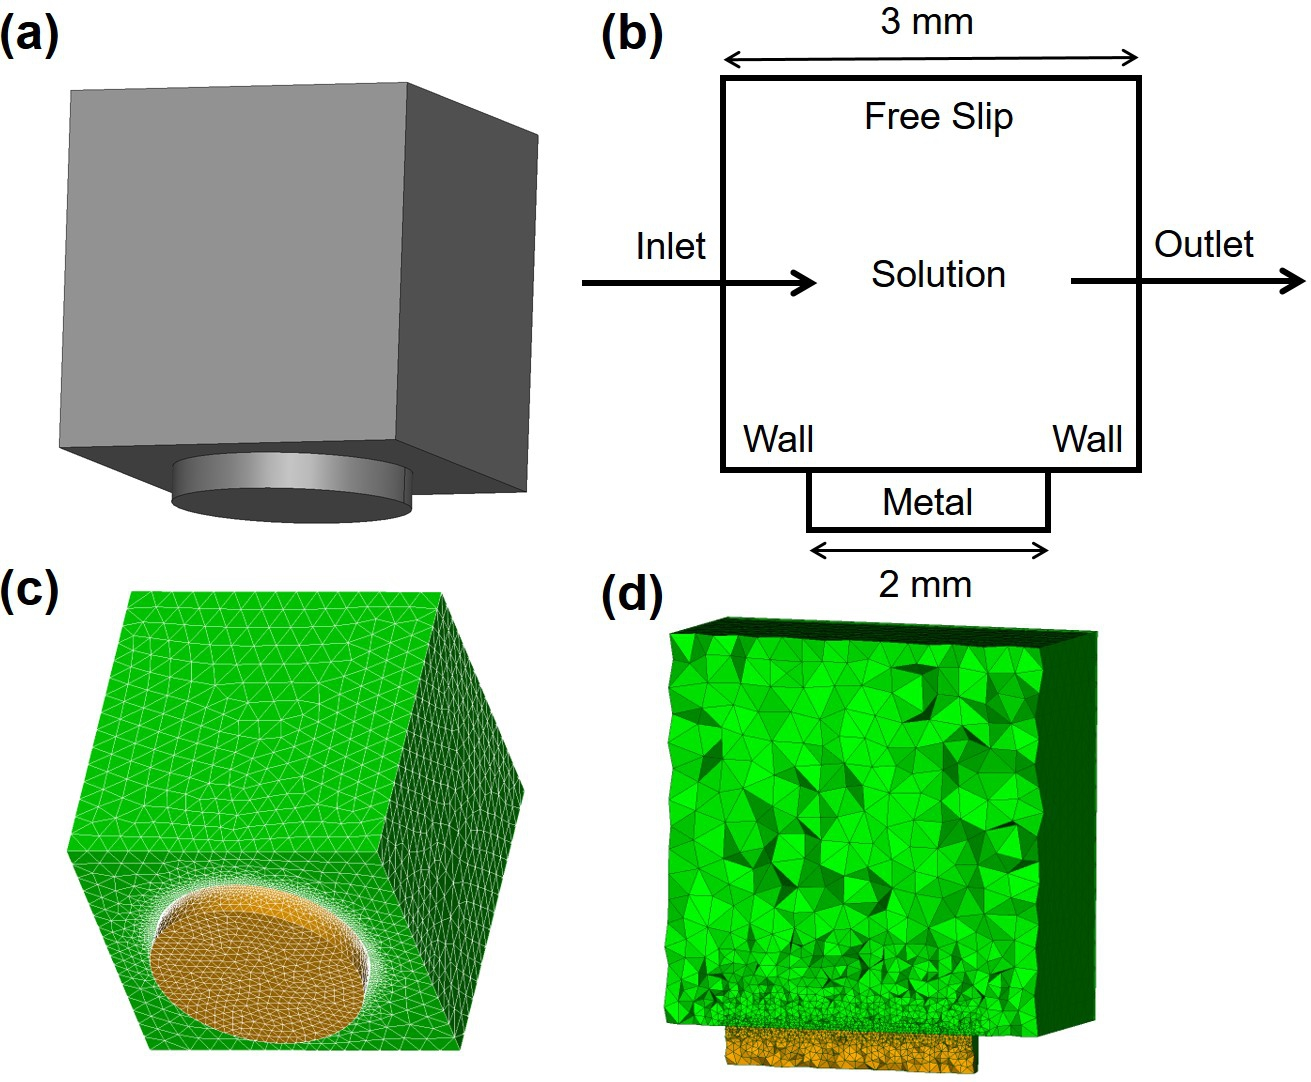
\includegraphics[width=\textwidth]{model_setup.jpg}
\caption[Computational model setup for local pH simulations]{Computational model setup for local pH simulations: a) the geometry of the desired domain, being a small portion of the full chamber on top of the disc-like sample, b) the dimensions of the domain and applied boundary conditions for the fluid flow simulation, c) the generated computational mesh, depicting the flow region in green and the biodegradable sample in yellow, d) a cross-section of the mesh showing the refined meshing on the interface of the degradable metal.} \label{fig:kinetics_model_setup}
\end{figure}

The boundary conditions include an inlet on the left of the box, an outlet on the right, a wall on the bottom except where the degrading part exists, and a free slip on top. The inlet velocity was selected to be a linear profile ranging from zero on the bottom to $1.0 \text{mm.s}^{-1}$ on the top, a value coming from solving the Navier-Stokes equations in the full chamber model (described in Chapter \ref{ch:fluid}).

The values of model parameters were set based on our previous work \cite{Barzegari2021}, but the following assumptions were also applied for selecting the proper parameters of the coupled computational model:
\begin{enumerate}
\item
Diffusion rate of hydroxide ions is 5-10 times more than the rate of Mg ions, so $D_{\mathrm{OH}}$ was set as $D_{\mathrm{OH}} = 7.5 D_{\mathrm{Mg}}$ \cite{Gonzalez2021}.
\item
The hydroxyapatite-like precipitation does not form immediately at the beginning and emerges later \cite{Gonzalez2021,Wang2022}. In the current model, it is set to start forming after the first hour of simulation time.
\item
The magnesium hydroxide layer is ticker at $37^{\circ}C$ \cite{Wang2022}, so the film elimination parameter ($k_2$) was set to be 50 times lower in this temperature in comparison to the room temperate.
\end{enumerate}

The density of the electrolyte was selected to be $1.085\times10^{-3} \text{g.mm}^{-3}$, and the dynamic viscosity was set to $1.28\times10^{-3} \text{g.mm}^{-1}\text{s}^{-1}$. The simulations were carried out on the Snellius supercomputer using 100 \gls{CPU} cores on a thin node with 256 GB of total memory.


\section{Results}

\subsection{Thermodynamics-based simulation}

Inputting the experimental conditions in the Hydra-Medusa software, including the initial composition of the electrolyte, temperature and the contributing chemical components, results in a big and complex output containing all the possible occurring chemical reactions. From this output, relevant reactions for the current biodegradation systems were filtered out, and the filtered reactions were converted to desired concentration units. Fig. \ref{fig:kinetics_medusa_profiles} depicts the output of this process separately for simulations performed at $25^{\circ}C$ (\gls{RT}) and $37^{\circ}C$, showing how the concentration of relevant components varies with changing the environment pH. The solubility products of these simulations were taken from Table \ref{tab:kinetics_reactions}, and equilibrium concentrations were set to be equal to the electrolyte composition, listed in Table  \ref{tab:kinetics_electrolyte_composition}. These results (module 2) were used by the linking module (module 3) to provide equilibrium information for the mechanistic model (module 1).

\begin{figure}[h]
\centering
\medskip
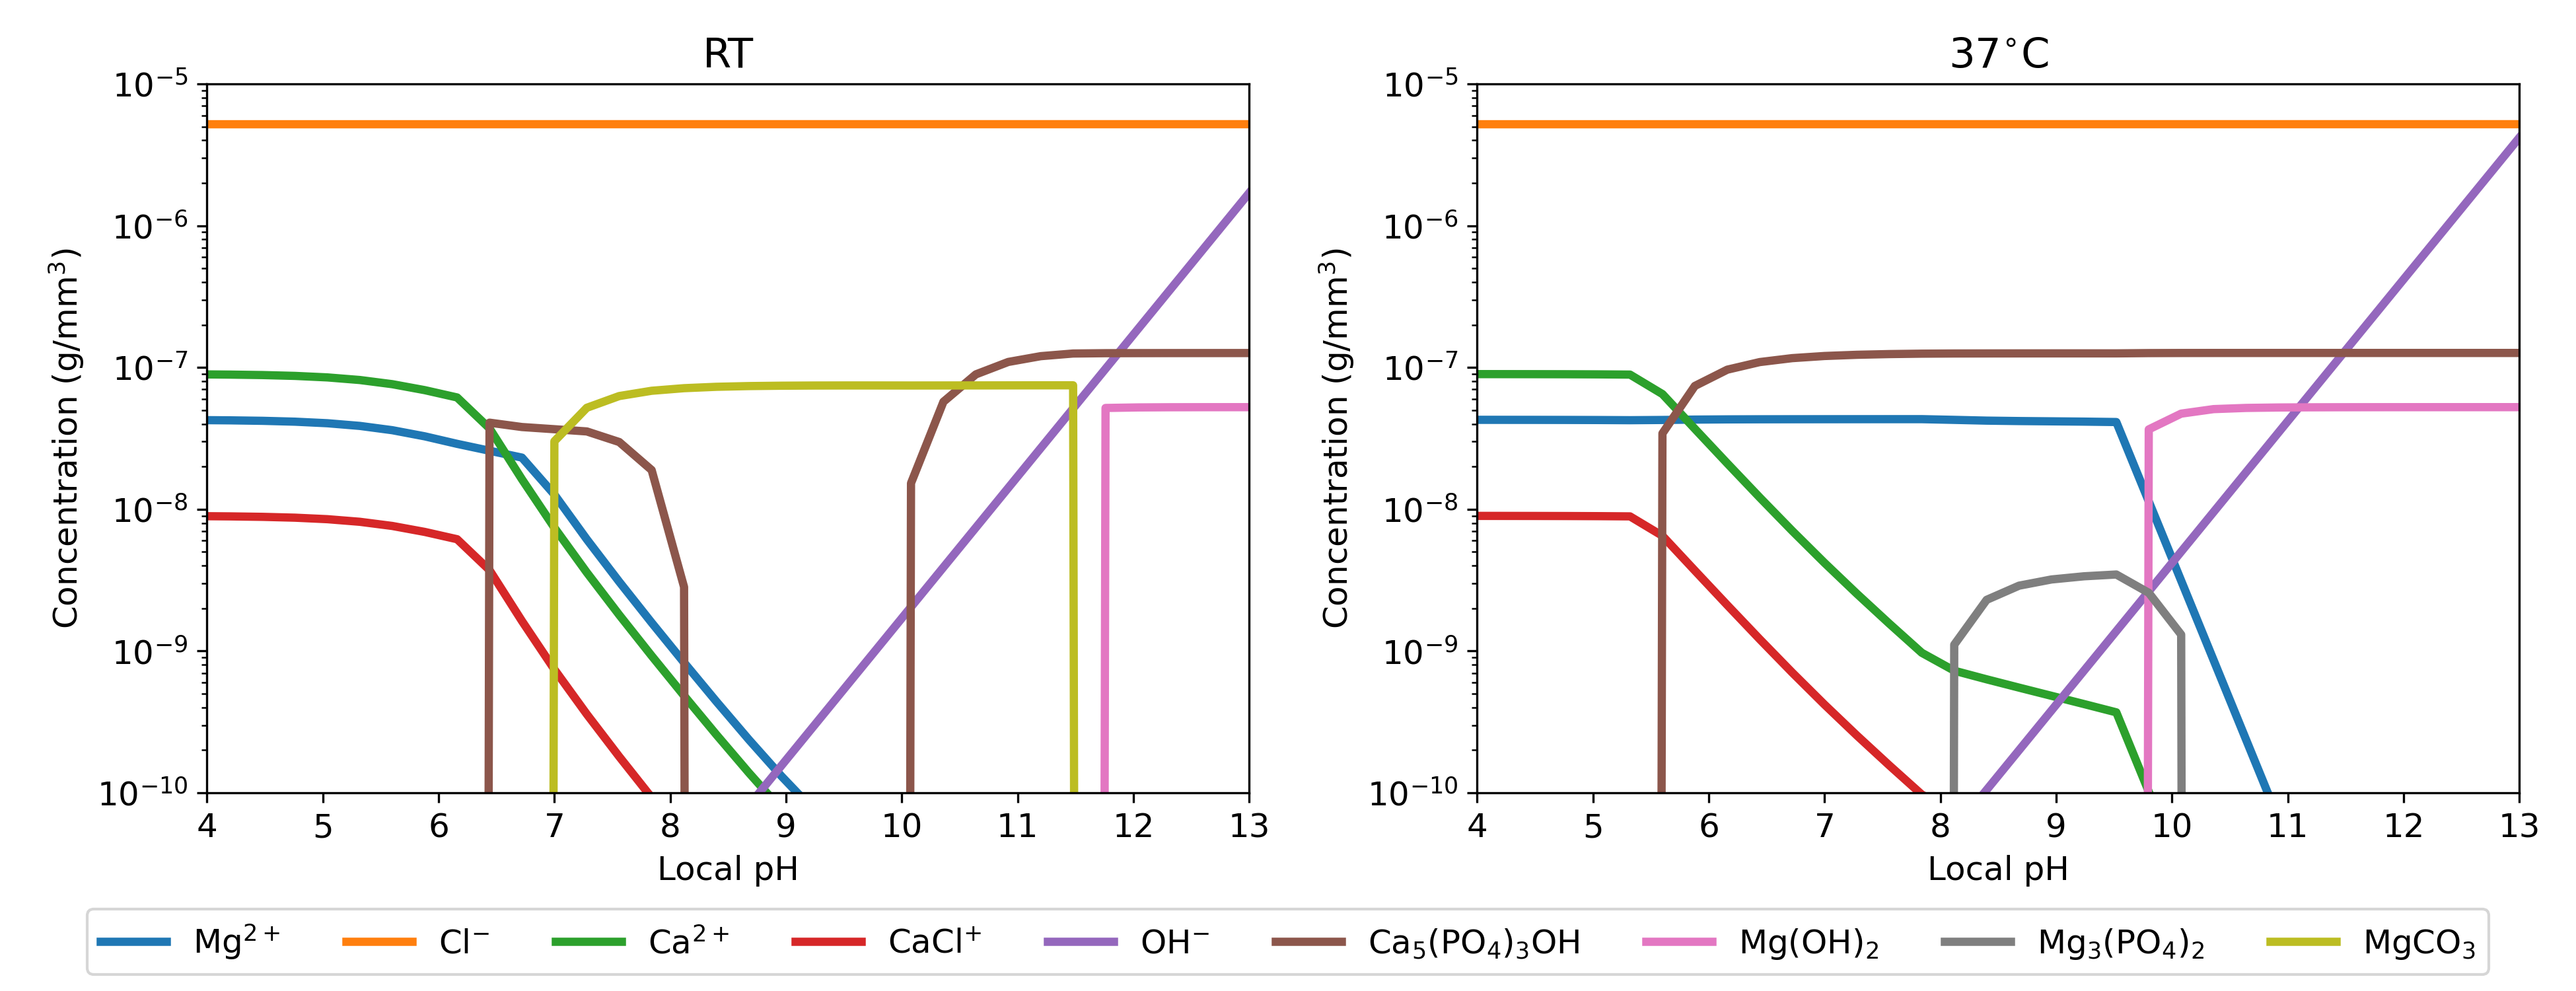
\includegraphics[width=\textwidth]{medusa_profiles.png}
\caption[Hydra-Medusa software output for given experimental conditions]{Selected relevant components from the Hydra-Medusa software output for given experimental conditions, showing how the concentration of various components vary with changing local pH} \label{fig:kinetics_medusa_profiles}
\end{figure}

\subsection{Biodegradation simulations}

In the current study, the local pH profiles, i.e., the pattern of pH changes in the region close to the degradation surface, were used to validate the developed coupled computational model. The comparison between computational predictions and experimental results was made in 3 different ways: 1) qualitative comparison of pH distribution above the degradable metal in a sample-centered square with an edge size of $3 \text{mm}$, 2) comparing the horizontal pH profiles, where the pH was measured over a line parallel to the sample, and 3) comparing vertical pH profiles, in which the pH was measured over a distance from the surface of the sample to the bulk of the electrolyte.

Fig. \ref{fig:kinetics_local_ph_visual} shows a visualization of the local pH profiles from the top and side views for simulations performed at  $25^{\circ}C$ (\gls{RT}) and $37^{\circ}C$ after 12 hours. These patterns are comparable with the local pH distribution measured in the experiments, as shown in Fig. \ref{fig:kinetics_local_ph_experimental}. In these figures, the flow is from left to right, advecting the released ions in the flow direction.

\begin{figure}[h]
\centering
\medskip
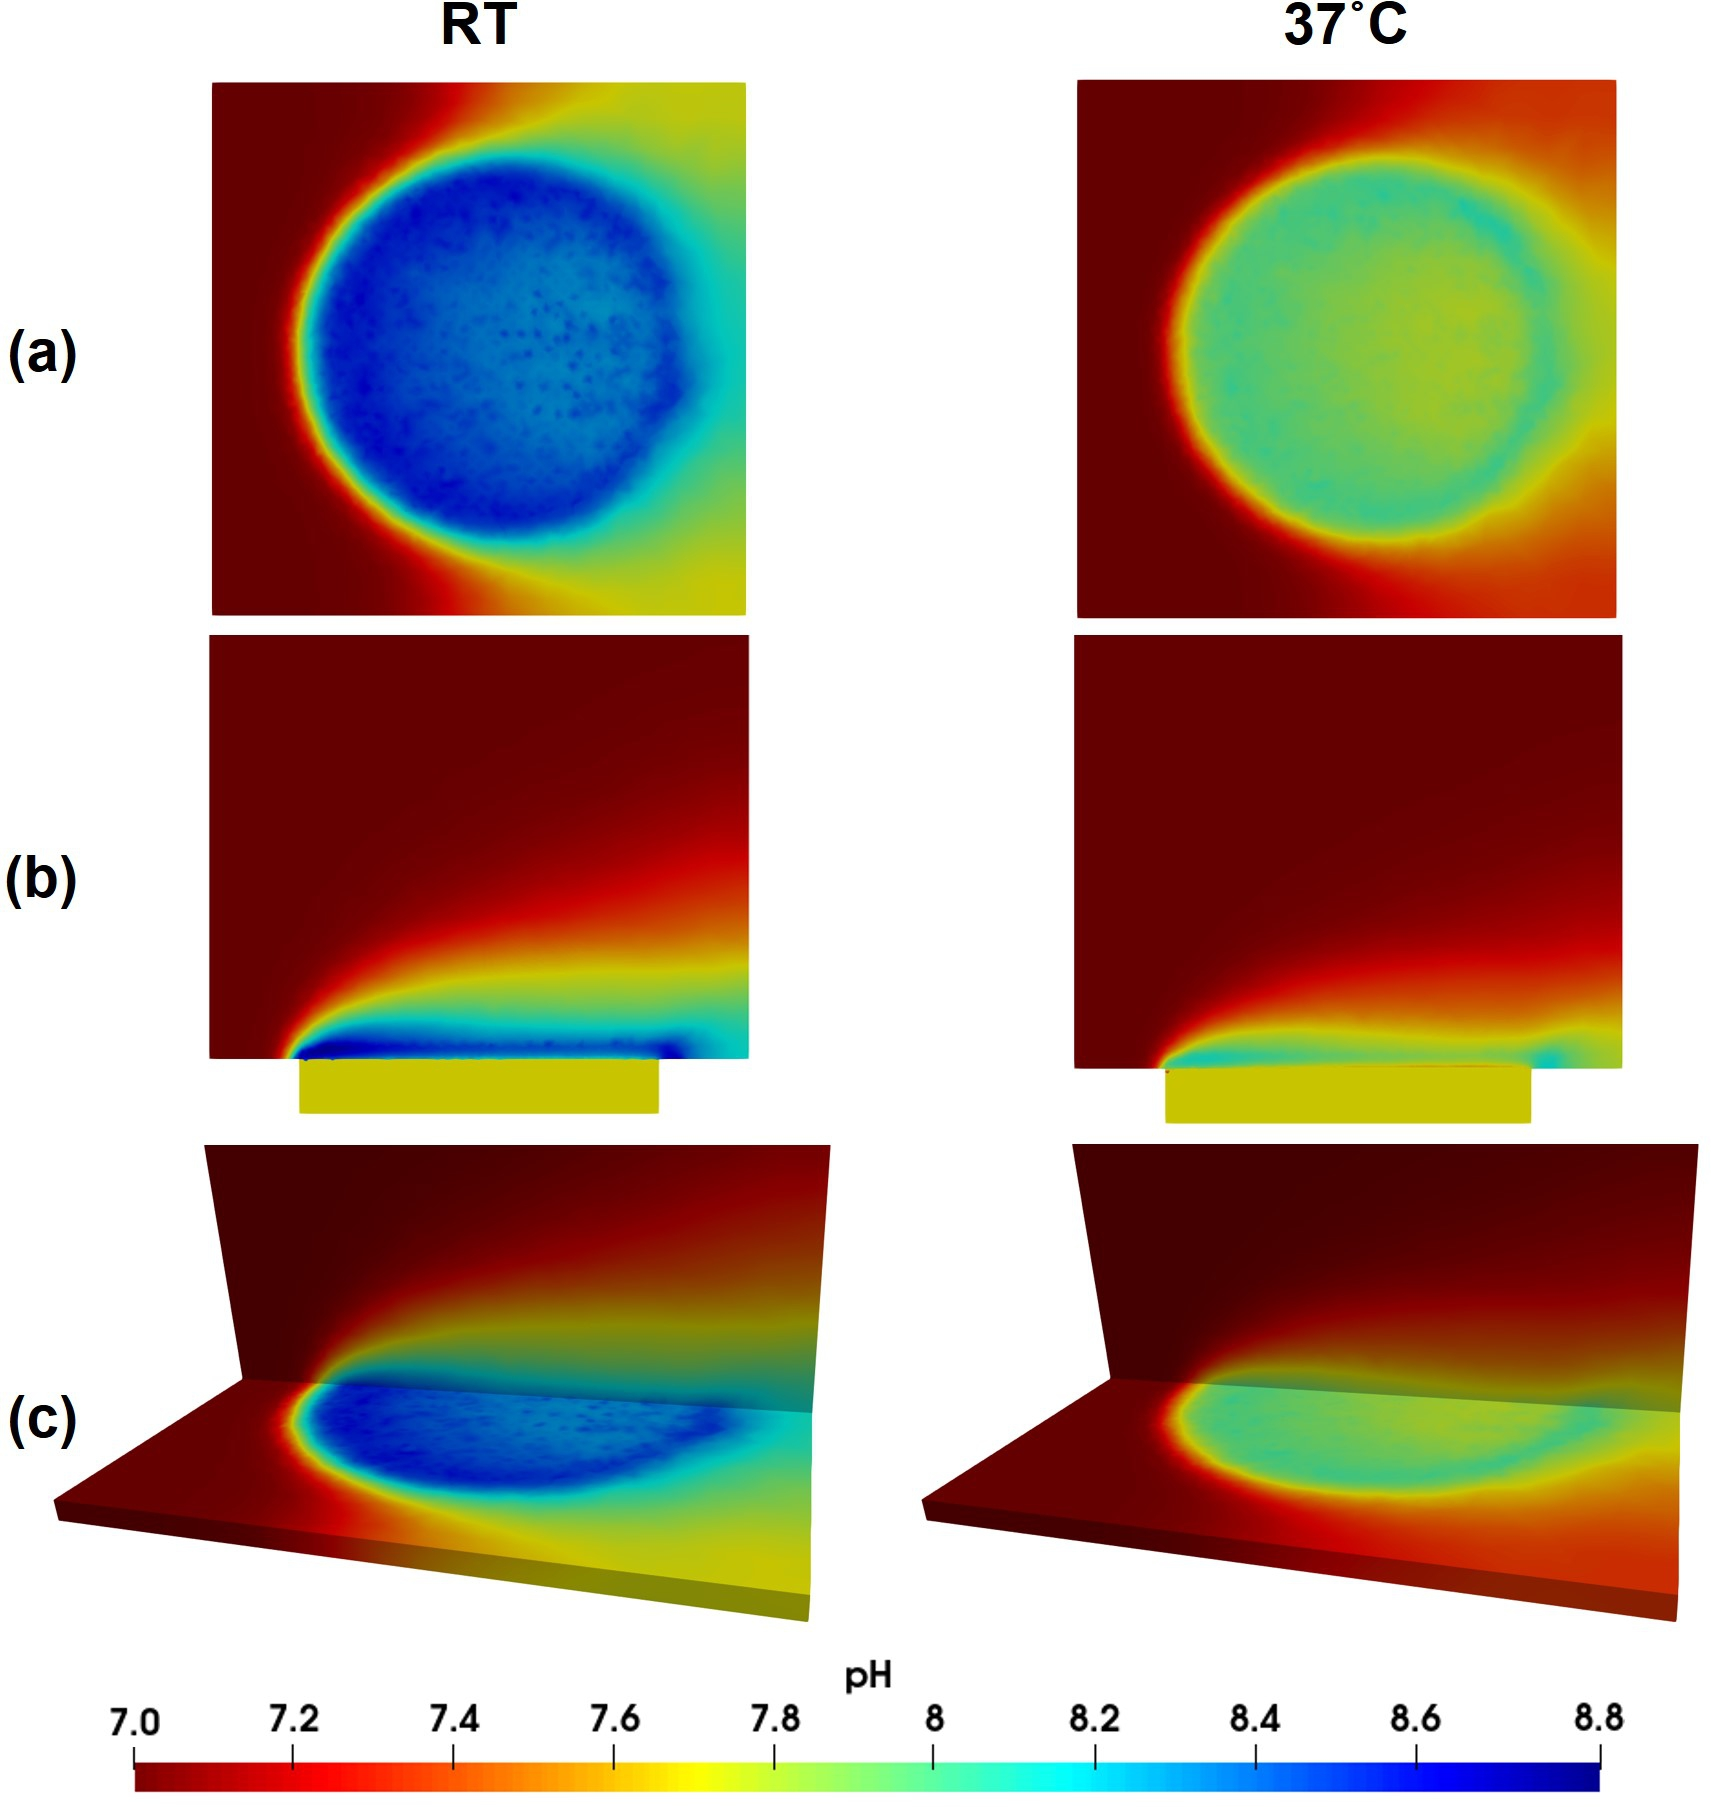
\includegraphics[width=\textwidth]{local_ph_visual.jpg}
\caption[Simulation results for local pH predictions]{Simulation results for local pH predictions, depicting the local pH in a) top view from a horizontal cross-section, b) side view from a vertical cross-section, and c) perspective view with both the top and side cross sections, for simulations performed at $25^{\circ}C$ (\gls{RT}) and $37^{\circ}C$.} \label{fig:kinetics_local_ph_visual}
\end{figure}

\begin{figure}[h]
\centering
\medskip
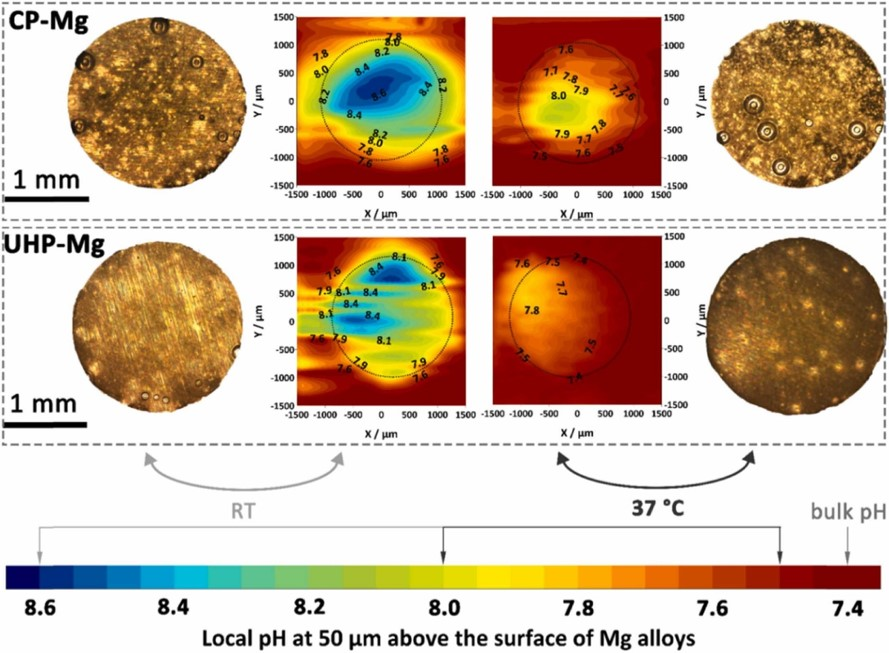
\includegraphics[width=\textwidth]{local_ph_experimental.jpg}
\caption[Experimental results for the distribution of local pH above the sample]{Experimental results for the distribution of local pH above the surface of the sample, measured after 12 hours of degradation.} \label{fig:kinetics_local_ph_experimental}
\end{figure}

Quantitative profiles provide a more accurate comparison between the computational predictions and experimentally-obtained values. The horizontal profiles, also called line scans, are depicted in Fig. \ref{fig:kinetics_vertical_profile}, in which the local pH changes are plotted over a horizontal line located $50 \mu\mathrm{m}$ above the surface of the sample. The profiles are shown separately for the experiments performed with \gls{CP} and \gls{UHP} Mg and the computational model. The results were recorded after 3, 6, and 12 hours of immersion.

\begin{figure}[h]
\centering
\medskip
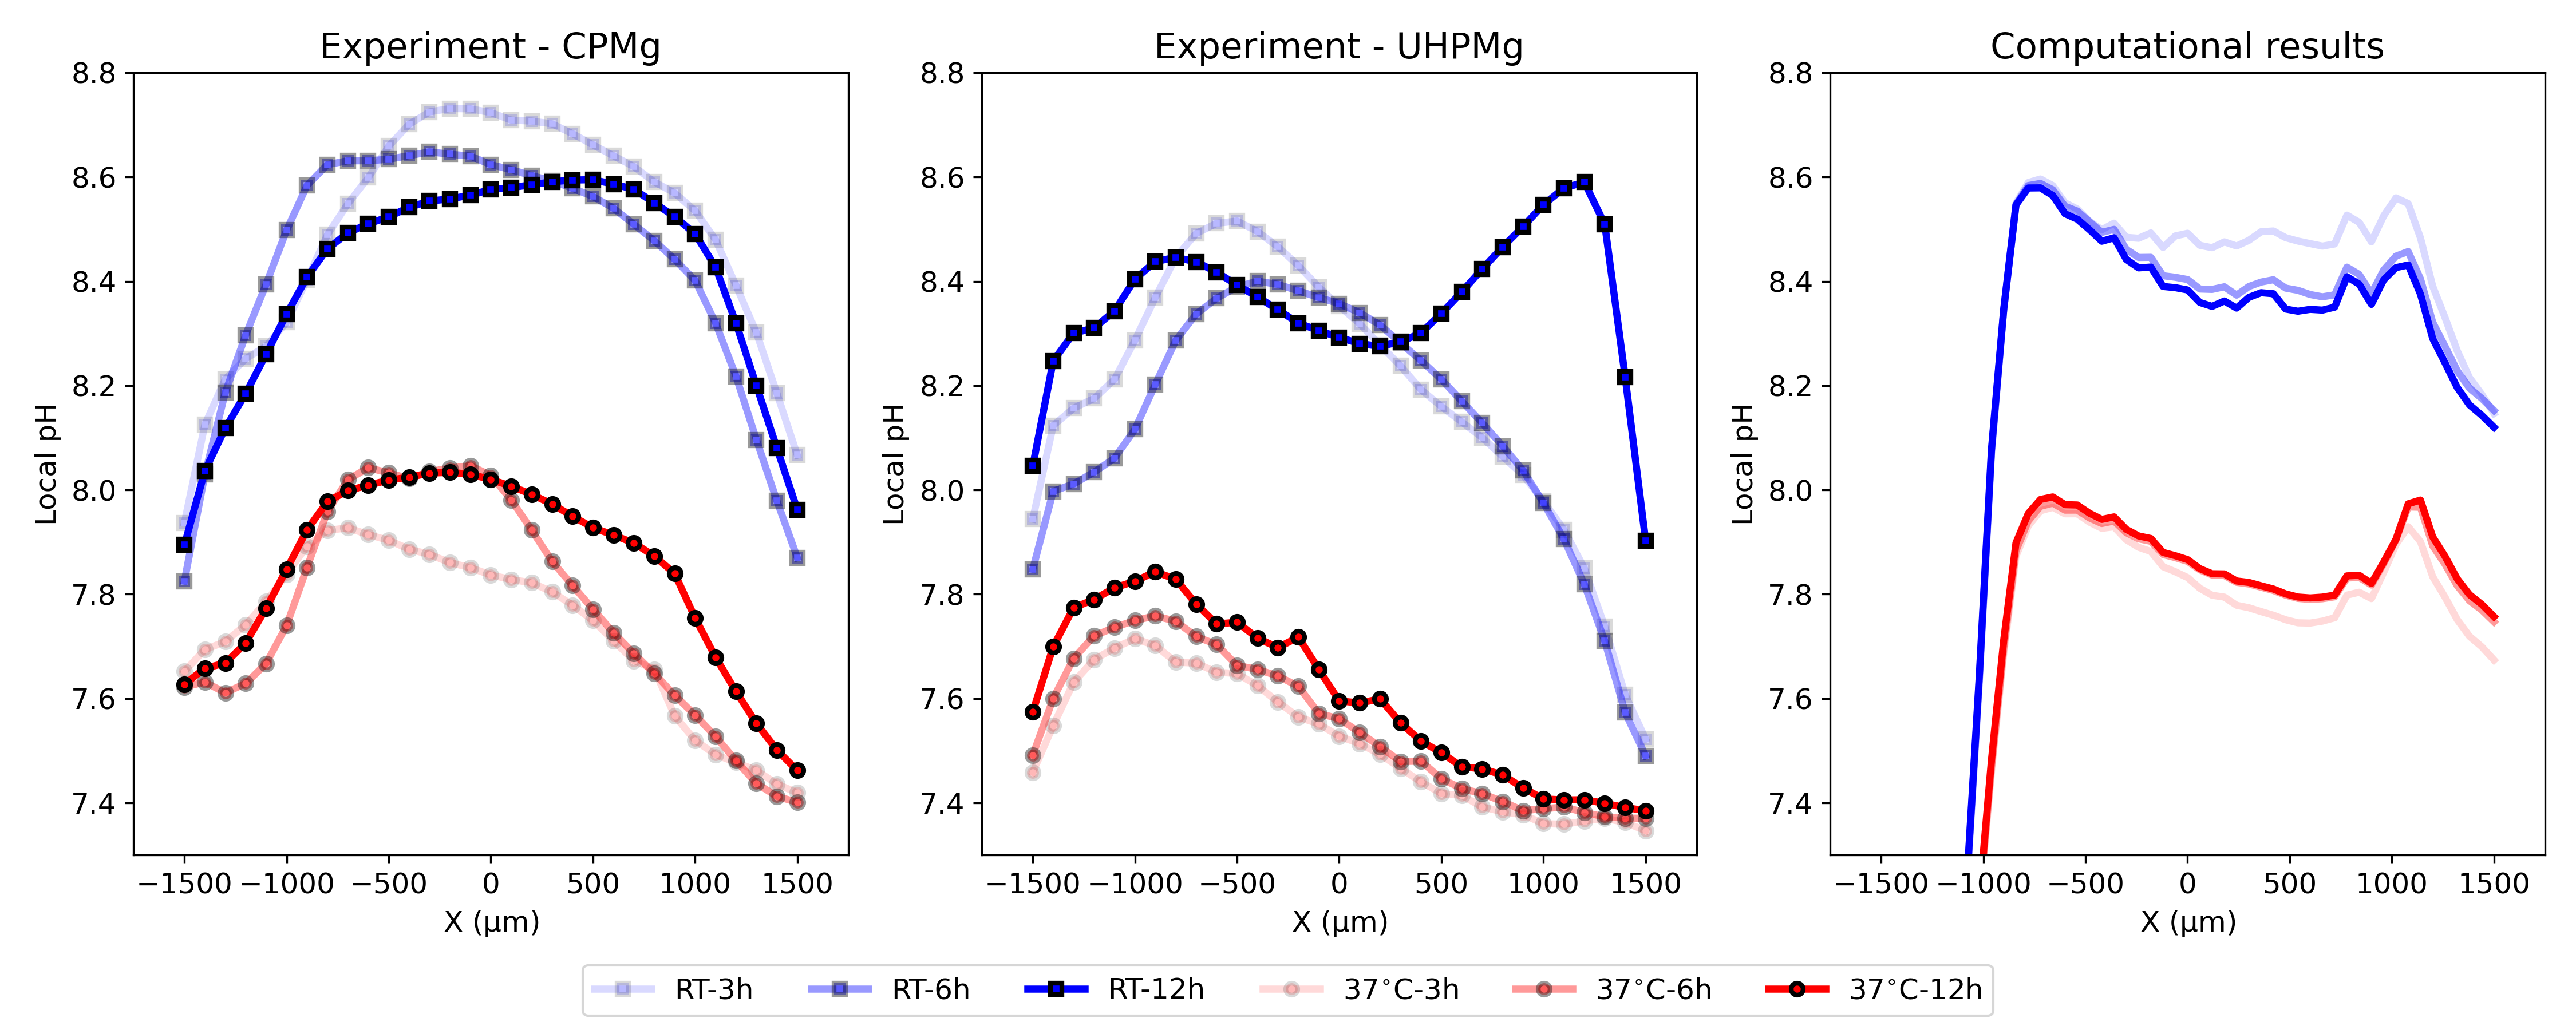
\includegraphics[width=\textwidth]{line_scans.png}
\caption[Comparing computational and experimental for horizontal line scans of local pH]{Comparing computational predictions and experimentally-obtained horizontal line scans of local pH changes, measured $50 \mu\mathrm{m}$ above the surface of the sample after 3, 6, and 12 hours of degradation.} \label{fig:kinetics_line_scans}
\end{figure}

Similarly, Fig. \ref{fig:kinetics_vertical_profile} shows the vertical pH profile after 12 hours of degradation, which was the final time of the simulation. The local pH is measured over a distance of $0.5 \mathrm{mm}$ vertically, starting from $50 \mu\mathrm{m}$ above the sample.

\begin{figure}[h]
\centering
\medskip
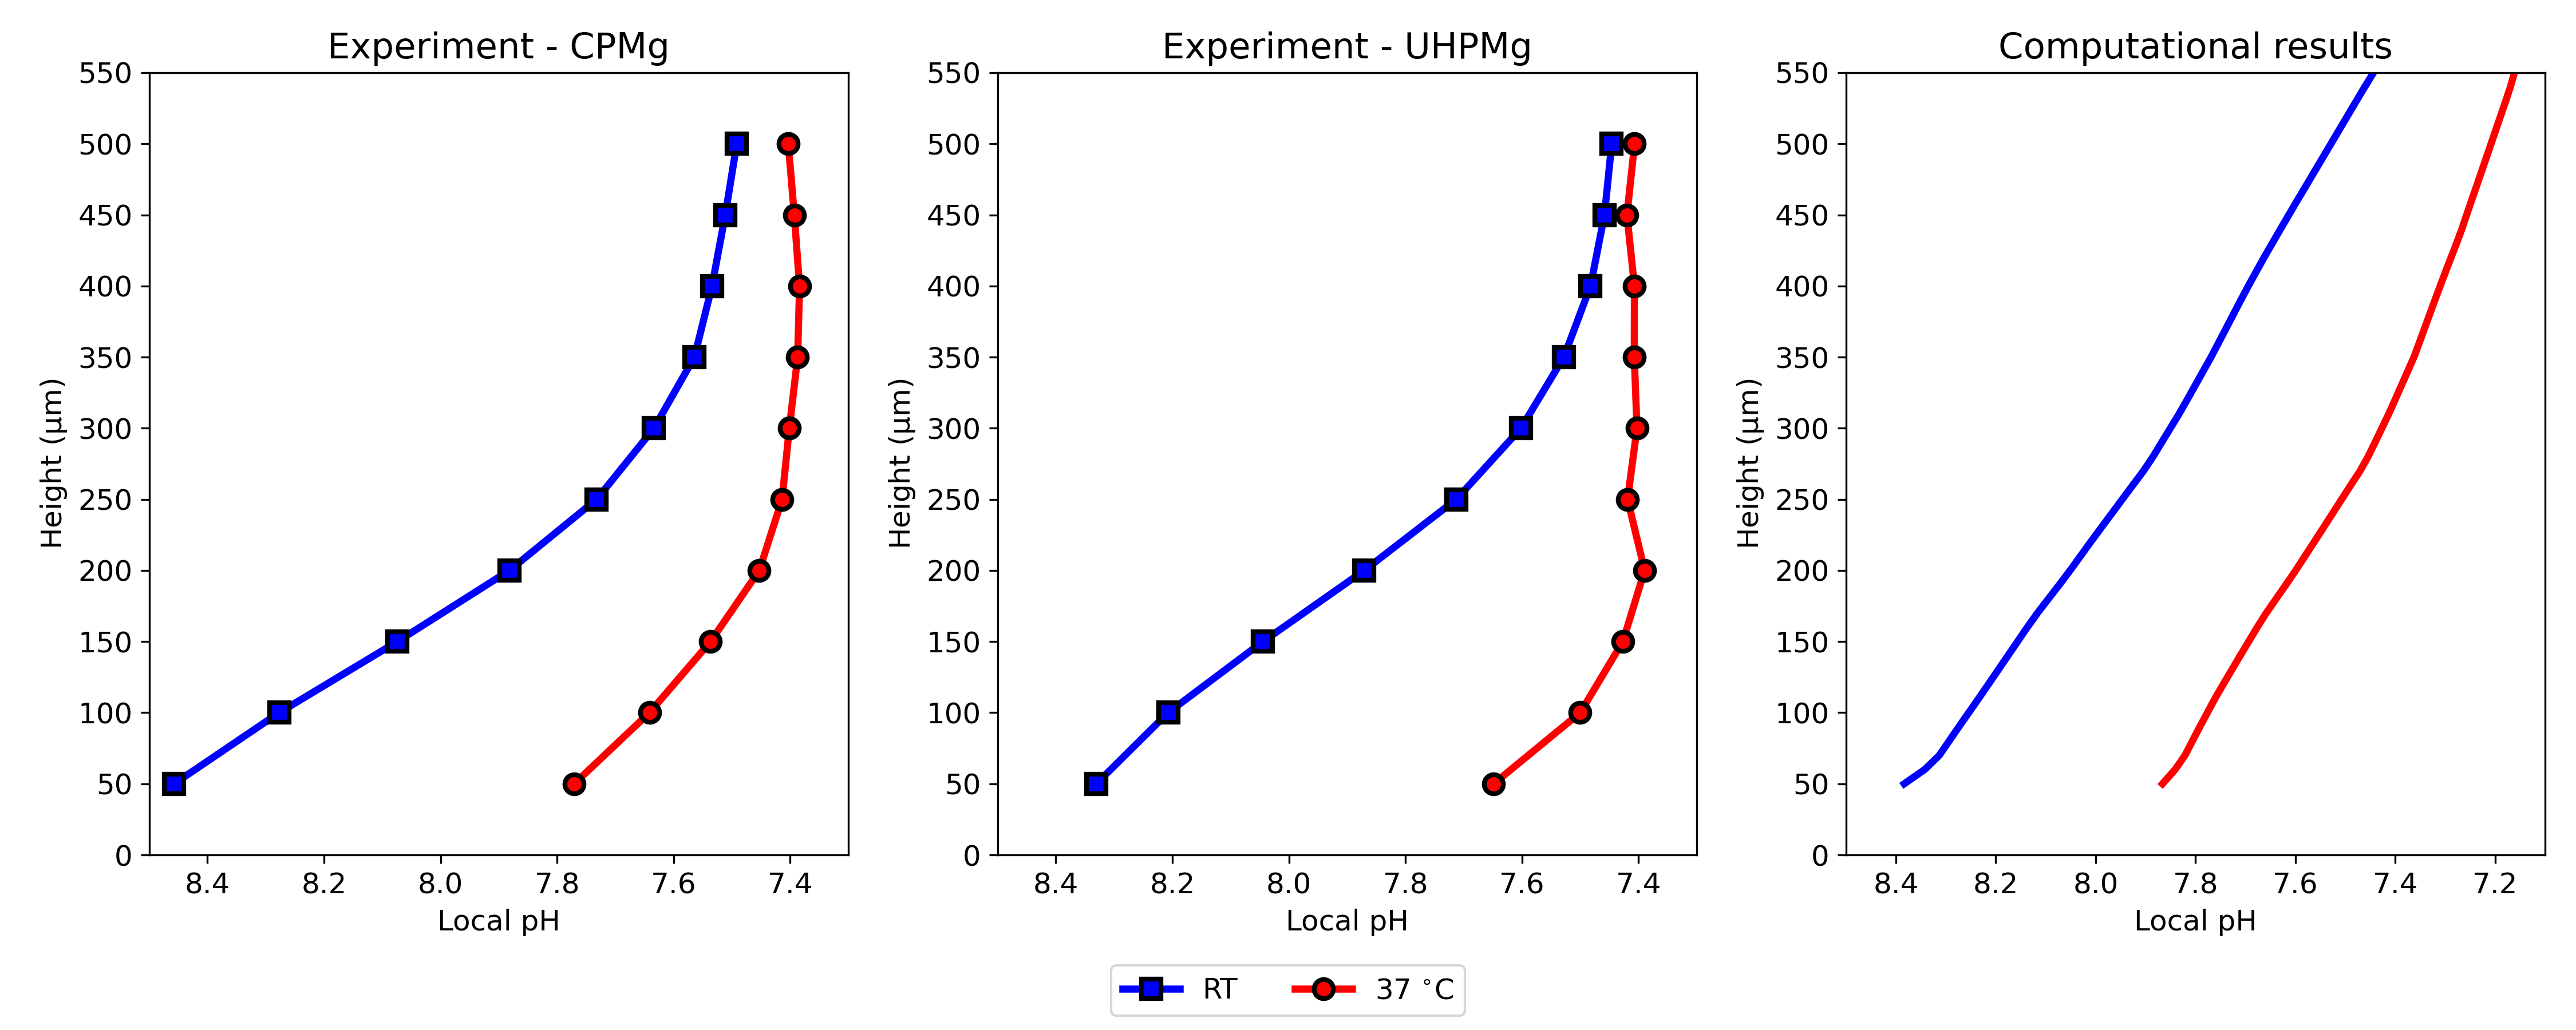
\includegraphics[width=\textwidth]{vertical_profile.png}
\caption[Comparing computational and experimental vertical pH profiles]{Comparing computational and experimental results for the local pH profiles, measured over a vertical line above the center of the sample after 12 hours of immersion.} \label{fig:kinetics_vertical_profile}
\end{figure}

\section{Discussion}

In this study, an interface-coupled multiphysics biodegradation model was developed in order to predict the corrosion behavior in simulated body fluids in the presence of various chemical components. The quantity to compare with the experimental results was the predicted local pH, which reflects the capabilities of the model to capture the complex chemistry occurring near the biodegradation interface. For this end, our previous biodegradation model \cite{Barzegari2021} was extended and coupled with a fluid flow model capturing the hydrodynamics condition. Then, the coupled model was linked to a thermodynamics-based code for computing the concentration of involved chemical components, the results of which were provided back to the biodegradation model via a linking module to compute the concentration of the precipitation layer.

It has been shown that the local pH changes can be a reflective characteristic of the biodegradation process in \gls{SBF}-like solutions \cite{Gonzalez2021,Wang2022}. Consequently, the vertical and horizontal local pH profiles can be reasonably used for the validation of the computational models of the biodegradation process. Capturing the complex interaction of various chemical components on the biodegradation interface in a mechanistic model can be a big challenge, especially for 3D cases with any arbitrary shape. That's why several interfaces were coupled in the current study to deliver such a model.

In this work, while the experiments were performed using \gls{CP} and \gls{UHP} Mg, the computational model does not take into account the difference in the elemental composition of these materials. Instead, the biodegradation model was developed by ignoring the effect of alloying elements and impurities. The variation in the obtained experimental results, such as different behavior of \gls{CP} and \gls{UHP} for horizontal pH profiles in line scan mappings (Fig. \ref{fig:kinetics_line_scans}) and distribution of local pH above the sample (Fig. \ref{fig:kinetics_local_ph_experimental}), supports this assumption and simplification. As a consequence, the computational results, including the pH profiles (Fig. \ref{fig:kinetics_vertical_profile}), line scans (Fig. \ref{fig:kinetics_line_scans}), and local pH distributions (Fig. \ref{fig:kinetics_local_ph_visual}), lies between the values and profiles obtained for \gls{CP} and \gls{UHP} Mg.

Recent studies on measuring local pH changes on the biodegradation surface of Mg alloys show that the local values are different from the pH within the bulk of the electrolyte \cite{Gonzalez2021}. For example, in the tests performed by Mareci et al. \cite{Mareci2016}, such observation was made when the vertical pH profiles were compared to the global pH values. Similar behavior was observed in the Wang et al. work \cite{Wang2022}. Reproducing this behavior is problematic in mechanistic computational models due to the uniformity of the diffusion of hydroxide ions that change the pH. In other words, a uniform diffusion with a relatively high diffusion coefficient leads to the same local and global pH values. In the model presented here however, spatially dependent  behavior was successfully reproduced \textit{in silico} by letting a narrow film form at the beginning of the mechanistic biodegradation simulation and then computing the interaction of various ions in this narrow region by using the coupled thermodynamics-based code. Comparing the results of the predicted vertical pH profiles with the experimentally obtained curves (Fig. \ref{fig:kinetics_vertical_profile}) shows good agreement, implying that the employed approach was able to mimic the complex chemistry on the biodegradation surface from a quantitative point of view. Yet, a different behavior can be observed further away from the surface where the local pH approaches the global value. In experimental results, this happens at a shorter distance from the implant compared to the computational predictions (Fig. \ref{fig:kinetics_vertical_profile}) where yielding to the global pH seems to occur at longer distances from the biodegradation surface. This behavior can be confirmed by the visualization of computed pH (Fig. \ref{fig:kinetics_local_ph_visual}) and is due to the uniform diffusion mechanism of ions in the computational model, causing a gradient in the bulk part outside of the narrow formed region.

The results of horizontal line scan mapping on the surface of the sample and local pH distribution (Figs. \ref{fig:kinetics_line_scans} and \ref{fig:kinetics_local_ph_experimental}) show that the pH starts to change in regions above the sample. In the computational predictions depicted in Fig. \ref{fig:kinetics_line_scans}, the change of pH starts sharply when the line scan reaches the sample, a behavior rooted in the presence of the fluid flow model, which prevents ions from being diffused to the left, as shown in Fig. \ref{fig:kinetics_local_ph_visual}. Similarly, the advected ions in the direction of fluid flow (to the right in Fig. \ref{fig:kinetics_local_ph_visual}) prevent the pH value from decreasing dramatically where the sample ends in the line scan mapping. Moreover, the line scans show different behavior for experiments performed at room temperature compared to $37^{\circ}\text{C}$, especially for \gls{CP} Mg samples. At \gls{RT}, the horizontal pH profile tends to descend slightly over time, meaning that the profile measured after 3 hours of degradation is placed above the one measured after 12 hours. This behavior occurs oppositely for the measurement done at $37^{\circ}\text{C}$. The computational predictions of line scan profiles follow the same pattern, which could be due to how the coupled model computed the change of concentration of various chemical components and their contribution to the change of local pH.

As mentioned before, various chemical components of the electrolyte contribute differently to the change of pH, among which $\mathrm{Ca}^{2+}$ seems to have the most intricate effect \cite{Willumeit-Roemer2019}. It has been reported that in the absence of $\mathrm{Ca}^{2+}$ ions, the surface pH tends to be between 10 and 11, the typical range for pH value in biodegradation tests performed in saline solution \cite{Gonzalez2021}. This value is in line with the computational predictions of our previous study \cite{Barzegari2021}. However, in presence of $\mathrm{Ca}^{2+}$ cations, local pH between 7.8 and 8.5 and significantly lower degradation rates are reported \cite{Mei2019,Gnedenkov2019,Tefashe2015,Lamaka2009}. These findings are in line with the predictions made by the model presented in this chapter, obtained by coupling a mechanistic modeling approach and chemical equilibrium modeling, the latter of which considers the presence of $\mathrm{Ca}^{2+}$.

Knowing the mechanism of ionic activities at regions close to the biodegradation interface is crucial for comprehending the chemical process of Mg in complex solutions such as simulated physiological conditions. The developed computational model can be seen as an a facilitating tool for moving towards understanding these mechanisms by making it possible to virtually investigate the effective parameters such as the flow rate and environment composition. This knowledge will be helpful for biomedical applications where new coating and stabilization systems can be developed for different implantation environments.

%\section{Data Availability}
%
%The data used in the paper are available from the authors upon request.
%
%\section{Code Availability}
%The source code of the programs used in this paper is available from the authors upon request.
%
%
%\section{Acknowledgements}
%
%\section{Author Contributions}
%
%\section{Competing Interests}


%%%%%%%%%%%%%%%%%%%%%%%%%%%%%%%%%%%%%%%%%%%%%%%%%%
% Keep the following \cleardoublepage at the end of this file,
% otherwise \includeonly includes empty pages.
\cleardoublepage
